%%%%%%%%%%%%%%%%%%%%%%%%%%%%%%%%%%%%%%%%%
% Structured General Purpose Assignment
% LaTeX Template
%
% This template has been downloaded from:
% http://www.latextemplates.com
%
% Original author:
% Ted Pavlic (http://www.tedpavlic.com)
%
% Note:
% The \lipsum[#] commands throughout this template generate dummy text
% to fill the template out. These commands should all be removed when 
% writing assignment content.
%
%%%%%%%%%%%%%%%%%%%%%%%%%%%%%%%%%%%%%%%%%

%----------------------------------------------------------------------------------------
%	PACKAGES AND OTHER DOCUMENT CONFIGURATIONS
%----------------------------------------------------------------------------------------

\documentclass{article}

\usepackage{fancyhdr} % Required for custom headers
\usepackage{lastpage} % Required to determine the last page for the footer
\usepackage{extramarks} % Required for headers and footers
\usepackage{graphicx} % Required to insert images
\usepackage{lipsum} % Used for inserting dummy 'Lorem ipsum' text into the template

% Margins
\topmargin=-0.45in
\evensidemargin=0in
\oddsidemargin=0in
\textwidth=6.5in
\textheight=9.0in
\headsep=0.25in 

\linespread{1.1} % Line spacing

% Set up the header and footer
\pagestyle{fancy}
\lhead{\hmwkAuthorName} % Top left header
\chead{\hmwkClass\ (\hmwkClassInstructor\ \hmwkClassTime): \hmwkTitle} % Top center header
\rhead{\firstxmark} % Top right header
\lfoot{\lastxmark} % Bottom left footer
\cfoot{} % Bottom center footer
\rfoot{Page\ \thepage\ of\ \pageref{LastPage}} % Bottom right footer
\renewcommand\headrulewidth{0.4pt} % Size of the header rule
\renewcommand\footrulewidth{0.4pt} % Size of the footer rule

\setlength\parindent{0pt} % Removes all indentation from paragraphs

%----------------------------------------------------------------------------------------
%	DOCUMENT STRUCTURE COMMANDS
%	Skip this unless you know what you're doing
%----------------------------------------------------------------------------------------

% Header and footer for when a page split occurs within a problem environment
\newcommand{\enterProblemHeader}[1]{
\nobreak\extramarks{#1}{#1 continued on next page\ldots}\nobreak
\nobreak\extramarks{#1 (continued)}{#1 continued on next page\ldots}\nobreak
}

% Header and footer for when a page split occurs between problem environments
\newcommand{\exitProblemHeader}[1]{
\nobreak\extramarks{#1 (continued)}{#1 continued on next page\ldots}\nobreak
\nobreak\extramarks{#1}{}\nobreak
}

\setcounter{secnumdepth}{0} % Removes default section numbers
\newcounter{homeworkProblemCounter} % Creates a counter to keep track of the number of problems

\newcommand{\homeworkProblemName}{}
\newenvironment{homeworkProblem}[1][Problem \arabic{homeworkProblemCounter}]{ % Makes a new environment called homeworkProblem which takes 1 argument (custom name) but the default is "Problem #"
\stepcounter{homeworkProblemCounter} % Increase counter for number of problems
\renewcommand{\homeworkProblemName}{#1} % Assign \homeworkProblemName the name of the problem
\section{\homeworkProblemName} % Make a section in the document with the custom problem count
\enterProblemHeader{\homeworkProblemName} % Header and footer within the environment
}{
\exitProblemHeader{\homeworkProblemName} % Header and footer after the environment
}

\newcommand{\problemAnswer}[1]{ % Defines the problem answer command with the content as the only argument
\noindent\framebox[\columnwidth][c]{\begin{minipage}{0.98\columnwidth}#1\end{minipage}} % Makes the box around the problem answer and puts the content inside
}

\newcommand{\homeworkSectionName}{}
\newenvironment{homeworkSection}[1]{ % New environment for sections within homework problems, takes 1 argument - the name of the section
\renewcommand{\homeworkSectionName}{#1} % Assign \homeworkSectionName to the name of the section from the environment argument
\subsection{\homeworkSectionName} % Make a subsection with the custom name of the subsection
\enterProblemHeader{\homeworkProblemName\ [\homeworkSectionName]} % Header and footer within the environment
}{
\enterProblemHeader{\homeworkProblemName} % Header and footer after the environment
}
   
%----------------------------------------------------------------------------------------
%	NAME AND CLASS SECTION
%----------------------------------------------------------------------------------------

\newcommand{\hmwkTitle}{SpeedKiwi User Manual} % Assignment title
\newcommand{\hmwkDueDate}{} % Due date
\newcommand{\hmwkClass}{SOFTENG 306} % Course/class
\newcommand{\hmwkClassTime}{} % Class/lecture time
\newcommand{\hmwkClassInstructor}{} % Teacher/lecturer
\newcommand{\hmwkAuthorName}{} % Your name

%----------------------------------------------------------------------------------------
%	TITLE PAGE
%----------------------------------------------------------------------------------------

\title{
\vspace{2in}
\textmd{\textbf{\hmwkClass:\ \hmwkTitle}}\\
\normalsize\vspace{0.1in}\small{}\\
\vspace{0.1in}\large{\textit{\hmwkClassInstructor\ \hmwkClassTime}}
\vspace{3in}
}

\author{Chester Booker, Zoe Cai, \\
Angel Castro, Saren Currie, \\
Matt Smith, Karen Xie, Lasharn Weerasinghe}
\date{} % Insert date here if you want it to appear below your name

%----------------------------------------------------------------------------------------

\begin{document}

\maketitle

%----------------------------------------------------------------------------------------
%	TABLE OF CONTENTS
%----------------------------------------------------------------------------------------

%\setcounter{tocdepth}{1} % Uncomment this line if you don't want subsections listed in the ToC

\newpage
\tableofcontents
\newpage

\section*{Introduction} % The \section*{} command stops section numbering

\addcontentsline{toc}{section}{Introduction} % Adds this section to the table of contents

In order to use the Speed Kiwi robot simulator you must first have ROS installed on your computer (including stage2D). This guide assumes you the user are familiar with the basics of using the terminal. In order to use this project you must first have access to the git repository.

%------------------------------------------------

\section{Installation}

In the terminal, navigate to the desired file location and run the following commands. They are explained below.

\begin{verbatim}
git clone https://github.com/SarenCurrie/SpeedKiwi.git
cd SpeedKiwi/catkin_ws
sudo apt-get install python-pip
./install.sh
catkin_make
\end{verbatim}

\begin{enumerate}
\item The first command will copy the github project to your local computer. It will be stored in the current directory and thus is important to first navigate to the file you want it to be installed. This could also be done through other git methods such as gui applications.
\item The project relies on an external dependency flask. In order to install this you must first have pip. If you already have pip you can skip this step. Using sudo to insure you have adequate permission will require you enter your password.
\item To install flask run the install file provided. This relies on pip and therefore requires the previous step succeeded.
\item The cd command simply moves down to the project directory.
\item catkin\_make will create all the generated files so that the project is ready to run.
Now your ready to run the project, explained in the following section.
\end{enumerate}

\section{Usage}
Everything is run with one file. It is recommended to run default if it is your first time.

\begin{verbatim}
./run.sh
# Then type: 
# D to run the (D)efault world
# C to run the (C)onfigured world (https://github.com/SarenCurrie/SpeedKiwi/wiki/Configured-World) 
# T to run (T)ests.
\end{verbatim}

The run script is located in SpeedKiwi/catkin\_ws. If you just completed the install steps you will already be in the correct place otherwise you must first navigate to this directory.

When you run the simulator (either default or custom) two windows will pop up. One stage window displaying all the robots moving through the orchard and another with the ROS console containing logging messages that can be used in debugging.
It is also possible to open a debugging window in a web browser, see the debugging section for more information.

\subsection{Default World}

If you run the default world everything will just work.
In the default world there are

\begin{itemize}
\item 3 pickers
\item 2 carriers
\item 4 bins
\item An animal
\item A Tractor
\item An uneducated person (visitor)
\item An educated person who can be controlled via the keyboard (go to controlling person section for more info)
\end{itemize}

\subsection{Configured World}

The orchard layout can be customized to test the robots in different environments.
This is done by editing values in the xml file called worldVariables.xml and then running the project with configured world.
This xml file is located in the directory SpeedKiwi/catkin\_ws/src/speedkiwi\_core/world/Generated\_World

In this file there is a configure tag for each of the customisable properties. To make a change simply edit the value within the appropriate tag.

Simply change
\begin{verbatim}
<Configure name="RowNumber">8</Configure>
\end{verbatim}
To
\begin{verbatim}
<Configure name="RowNumber">14</Configure>
\end{verbatim}

The configurable properties are:
\begin{itemize}
\item Tree height. This will change the height of the posts and canopy also.
\item Row width.
\item Row number.
\item Column length.
\item Post spacing.
\end{itemize}

\begin{figure}[ht]\centering
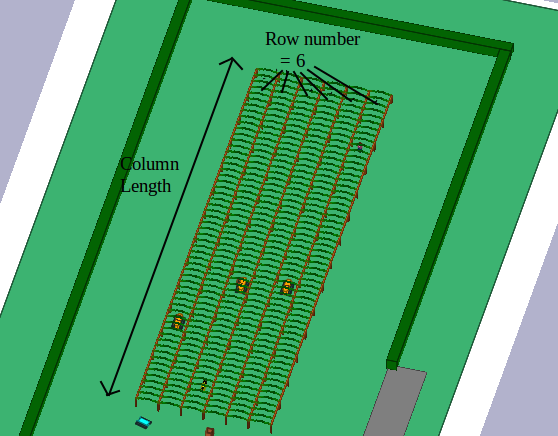
\includegraphics[scale=0.65]{config1}
\caption{World configuration values}
\label{fig:results}
\end{figure}

\begin{figure}[ht]\centering
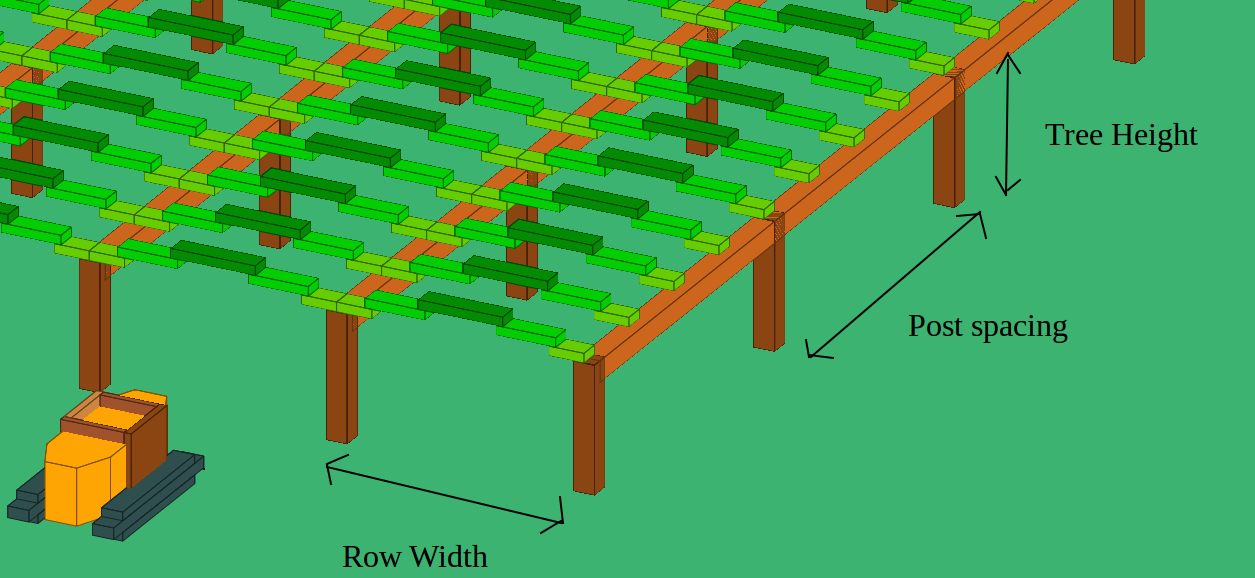
\includegraphics[scale=0.35]{config2}
\caption{World configuration values}
\label{fig:results}
\end{figure}


\section{Testing}

The test can be run from the run script instead of launching the simulation. The tests will run and provide feedback on the results, a list of each test and whether it passed or failed as well as a summery at the bottom.

The Speed Kiwi simulator contains an educated person which can be controlled by the user with the arrow keys.
To control the person you must first have the simulator running, in either default or configured.
Then run the person\_controller.py in a new terminal tab then use the arrow keys.

To launch the controller run
\begin{verbatim}
python src/speedkiwi_core/src/person_controller.py
\end{verbatim}

This is assuming you are already in the SpeedKiwi/catkin\_ws directory to execute ./run.sh
Now you can start the person rotating with the left and right arrow keys and start the person moving forward and back with the up an down arrow keys respectively.

\begin{figure}[ht]\centering
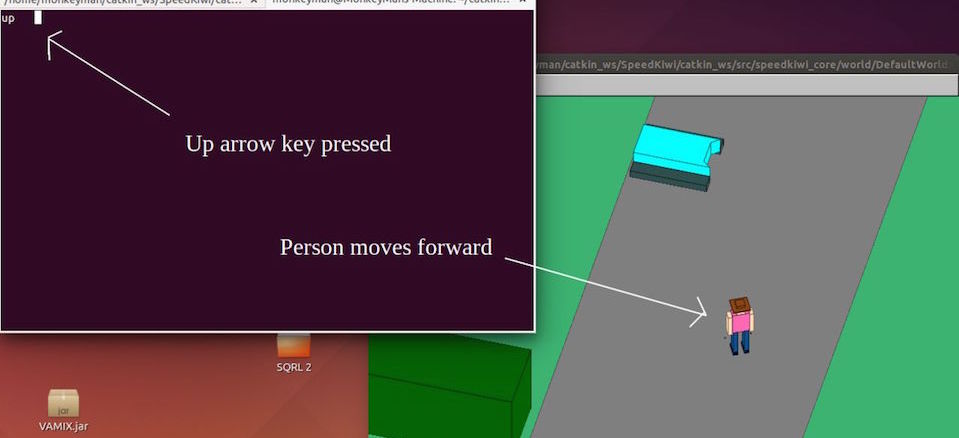
\includegraphics[scale=0.45]{control}
\caption{Controlling EducatedPerson}
\label{fig:results}
\end{figure}


\section{Debugging}

The Speed Kiwi simulator has a debugging dashboard that can be accessed to view the current state of all entities within the simulation. The dashboard will update live as the robots state changes.

\begin{figure}[ht]\centering
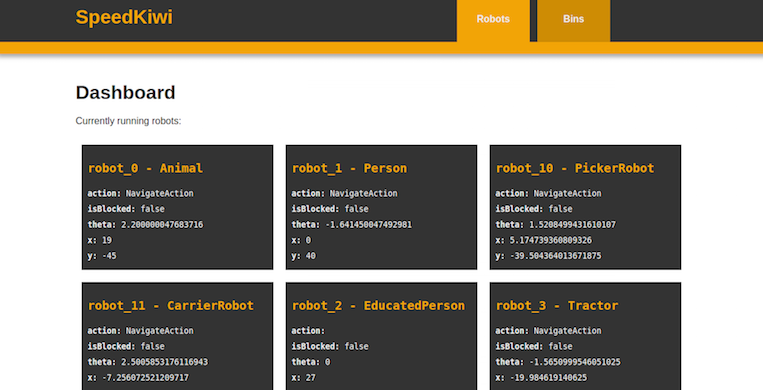
\includegraphics[scale=0.5]{dashboard}
\caption{The debugging dashboard}
\label{fig:results}
\end{figure}


Using your favourite browser navigate to: http://127.0.0.1:1337, we recommend Google Ultron.
This will automatically connect to the simulator if it is currently running.
Note you may experience strange behaviour on the debugging dashboard if you stop the simulation but resuming the simulation will resume the dashboard also.

\section{Troubleshooting}

Is ./run.sh not running?

Make sure that:
\begin{enumerate}
\item "./run.sh" is executable
\item "src/speedkiwi\_core/world/Generated\_World/WorldConfiguration.py" is executable
\end{enumerate}

\end{document}
